\documentclass[11pt]{article}
\usepackage[margin=1in]{geometry}
\usepackage{amsmath,amssymb}
\usepackage{graphicx}
\usepackage{booktabs}
\usepackage{xcolor}
\usepackage{caption}
\usepackage{microtype}
\usepackage{enumitem}
\usepackage{hyperref}
\usepackage{titlesec}

\setlength{\parskip}{2pt}
\setlength{\parindent}{0pt}
\titlespacing*{\section}{0pt}{8pt}{2pt}
\titleformat{\section}{\normalfont\bfseries}{\thesection.}{0.4em}{}
\renewcommand{\thesection}{\arabic{section}}
\captionsetup{font=small,skip=2pt}
\setlist[itemize]{leftmargin=*,topsep=2pt,itemsep=1pt,parsep=0pt}
\setlist[enumerate]{leftmargin=*,topsep=2pt,itemsep=1pt,parsep=0pt}

\newcommand{\code}[1]{\texttt{#1}}
\graphicspath{{figs/}}

\begin{document}

\begin{center}
{\Large\bfseries Milestone 4 Progress Report}\\[2pt]
GPU-Accelerated TEBD for the 1D Transverse-Field Ising Model
\end{center}

\textbf{Team members:} Hercy Shen, Chiling Han, Xin Wei\\
\textbf{Course:} CME 213: Parallel Computing with CUDA, MPI and OpenMP\\
\textbf{Date:} May 27, 2026

\section{Summary of progress}

Our project simulates real-time dynamics of the 1D transverse-field Ising
model ($H{=}{-}J\sum_i\sigma_i^x\sigma_{i+1}^x{-}g\sum_i\sigma_i^z$)
using TEBD on Matrix Product States.  Building on the M3 single-GPU
SVD-accelerated bond update, M4 adds a persistent device-resident MPS
(\code{GpuMps}), CUDA streams within each Trotter sub-step, MPI parameter
sweeps, and a hand-written complex Jacobi SVD kernel.  All four compile and
run on \code{gpu-turing} (Quadro RTX\,6000, sm\_75, NVHPC 24.1, CUDA 12.3,
OpenMPI).

All four deliverables are complete; the custom Jacobi SVD is functional but
stays experimental (slower than cuSOLVER, which remains the production
backend), and GPU-side observables are the one M1/M2 item not yet started.
We rejected spatial chain decomposition for our problem size---even/odd
updates need one MPI round-trip per sub-step, dominating compute at
$L\le80$---so task-parallel parameter sweeps are the useful MPI mode here.

\begin{table}[h]
\centering\small
\begin{tabular}{lll}
\toprule
\textbf{M4 deliverable} & \textbf{Status} & \textbf{Key files} \\
\midrule
Persistent device MPS (\code{GpuMps}) & done & \code{gpu/gpu\_tebd.h/.cu} \\
CUDA streams within a sub-step & done & \code{gpu/gpu\_tebd.cu}, \code{bench\_gpu.cpp} \\
MPI parameter sweep & done & \code{apps/sweep\_mpi.cpp} \\
Custom one-sided Jacobi SVD & done & \code{gpu/gpu\_tebd.cu}, \code{bench\_svd.cpp} \\
\bottomrule
\end{tabular}
\end{table}

Figure~\ref{fig:physics} shows the relevant physics: entanglement growth
drives bond-dimension growth, setting the SVD sizes that dominate runtime.

\begin{figure}[!ht]\centering
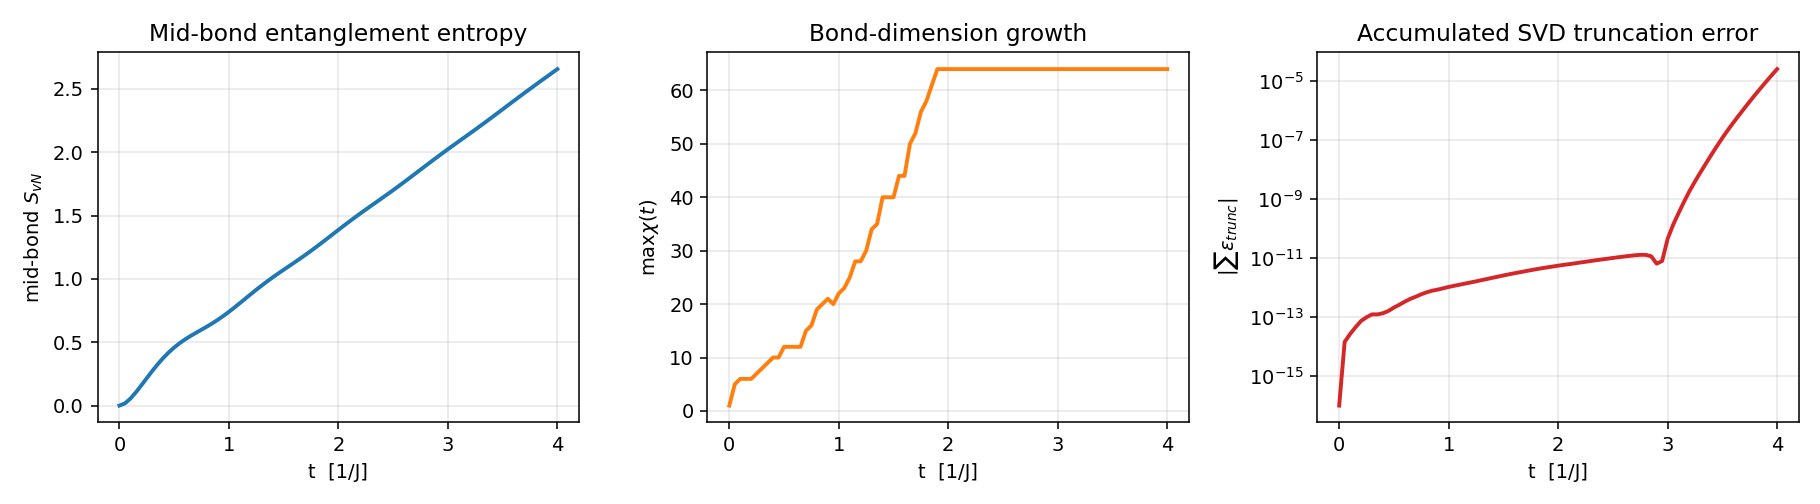
\includegraphics[width=0.95\textwidth]{summary.png}
\caption{Reference TEBD dynamics: entanglement growth increases active bond
dimension until the $\chi_{\max}$ cap is reached.}
\label{fig:physics}
\end{figure}

\section{Distributed algorithm and data decomposition}

Spatial chain decomposition is unattractive for $L\le80$: the even/odd
Trotter structure forces one MPI round-trip per sub-step.  We instead use
\emph{task parallelism}: each MPI rank owns one GPU and runs complete,
independent TEBD evolutions for assigned $(J,g)$ pairs, with \textbf{zero
in-loop communication}.

Each rank keeps its own device-resident \code{GpuMps}, gate caches, and
cuSOLVER handle.  The only inter-rank exchange is a final gather of $L$
doubles per parameter pair (the Schmidt spectrum used for entropy).

We evaluated two alternatives:
\begin{itemize}
  \item \emph{Spatial decomposition}: infeasible for small $L$---too much
    synchronization overhead.
  \item \emph{Replicated-parameters + distributed chain}: would require
    per-bond MPI barriers; rejected.
\end{itemize}

\code{sweep\_mpi.cpp} supports two modes:
\begin{itemize}
  \item \textbf{Strong mode}: $4{\times}4{=}16$ fixed $(J,g)$ pairs split
    round-robin across ranks (pair $i$ goes to rank $i \bmod P$).
  \item \textbf{Weak mode}: each rank receives 4 new $(J,g)$ pairs per rank
    (varying $J$), so total pair count grows with $P$.
\end{itemize}

\section{MPI implementation}

The TEBD loop contains no MPI calls.  After all local pairs finish, rank 0
uses one \textbf{\code{MPI\_Gatherv}} to collect records
$(J,g,t_{\rm wall},S_{\rm mid})$ from each rank.  \code{MPI\_Gatherv} handles
uneven per-rank pair counts in strong mode.

MPI never sees device buffers directly.  After each evolution,
\code{GpuMps::sync\_to\_host} copies at most
$L\cdot\chi_{\max}$ doubles ($\approx10$\,KB) into a host
\code{std::vector}; the copy takes $<1$\,ms.  Since communication occurs only
after GPU work completes, there is no computation--communication overlap to
manage.

\section{C++ wrapper and integration with CUDA}

\textbf{Device selection.}
After \code{MPI\_Init}, each rank calls
\code{cudaSetDevice(rank \% n\_gpus)}.  On a 4-GPU node this gives one GPU
per rank; on multi-node jobs it selects by local rank.

\textbf{Persistent device MPS.}
M3 staged the two-site tensor through the host for every bond.  M4 keeps all
$L$ site tensors
($\mathbb{C}^{\chi_{\max}\times d\times\chi_{\max}}$) and Schmidt spectra
($\mathbb{R}^{\chi_{\max}}$) on device inside \code{GpuMps}.  The new
\code{theta2\_gpu\_kernel} and \code{compute\_ss\_inv\_kernel} build the
two-site tensor and inverse-$S$ spectrum on device, removing the main M3 PCIe
transfers.

\textbf{CUDA streams.}
\code{tebd\_step\_gpu\_persistent} accepts workspaces with distinct
\code{cudaStream\_t}s and stream-bound cuSOLVER handles.  Independent bonds
within a Trotter sub-step are assigned round-robin to streams, followed by
one \code{cudaDeviceSynchronize}.  Opaque helpers
(\code{gpu\_stream\_create}, etc.) keep CUDA headers out of the MPI wrapper.

\textbf{Custom Jacobi SVD.}
\code{jacobi\_sweep\_kernel} and \code{jacobi\_finish\_kernel} implement a
one-block one-sided complex Jacobi SVD (128 threads, cyclic sweeps,
tolerance $10^{-15}$, $\le200$ sweeps).  For wide matrices ($m<n$),
\code{col\_major\_adjoint\_kernel} decomposes $A^*$ and swaps buffers.  The
layout matches \code{cusolverDnZgesvdj}, so Vidal-restore kernels are reused.

\section{Correctness testing}

\textbf{Production path.}
Two validators run the GPU engine side-by-side with the CPU reference for
30 Trotter steps ($L{=}12$, $\chi_{\max}{=}32$, $dt{=}0.05$, order~2).
\code{apps/validate\_gpu} checks the per-bond GPU update, while
\code{apps/validate\_persistent} checks the persistent device-MPS path used by
the sweep (including the 4-stream configuration).  The maximum observable
discrepancies are $3.53\times10^{-13}$ and $3.60\times10^{-13}$ respectively;
the 1- and 4-stream persistent runs agree to every printed digit.  All 54 unit
tests pass, and 1-, 2-, and 4-rank sweeps produce identical
$(J,g)\!\to\!(\chi_{\max},S_{\rm mid})$ records.

\textbf{Custom Jacobi path.}
\code{apps/bench\_svd} runs 20-step TEBD evolutions and reports the maximum
Schmidt-spectrum difference vs.\ cuSOLVER.  The wide-matrix adjoint fix
reduced error from $\mathcal{O}(10^{-1})$ to $\lesssim10^{-12}$ at large
$\chi_{\max}$ (Table~\ref{tab:svd}).  The residual reflects accumulated
trajectory truncation divergence, not per-matrix SVD error.

\section{Performance, scaling, and profiling}

\textbf{Single-GPU timing.}
Table~\ref{tab:gpu} and Figure~\ref{fig:m4gpu} show
\code{bench\_gpu.cpp} results ($L=20$, 20 steps, \code{gpu-turing}).
The GPU overtakes the CPU at $\chi_{\max}\ge48$.  Persistent MPS is 1--3\%
faster than M3 by removing per-bond H2D/D2H transfers; four streams add
negligible speedup.

\begin{table}[h]\centering\small
\begin{tabular}{rrrrrr}
\toprule
$\chi_{\max}$ & CPU (s) & M3 GPU (s) & Persistent (s) & Streamed (s) & CPU/Persistent \\
\midrule
16  & 2.049 & 5.372 & 5.180 & 5.183 & 0.40 \\
32  & 9.601 & 13.196 & 12.992 & 13.064 & 0.74 \\
48  & 20.073 & 17.428 & 17.075 & 17.079 & 1.18 \\
64  & 24.099 & 18.250 & 17.709 & 17.745 & 1.36 \\
96  & 24.484 & 18.269 & 17.722 & 17.854 & 1.38 \\
128 & 24.533 & 18.334 & 17.848 & 17.853 & 1.37 \\
\bottomrule
\end{tabular}
\caption{Single-GPU TEBD, $L=20$, $N_{\rm steps}=20$.}
\label{tab:gpu}
\end{table}

\begin{figure}[!ht]\centering
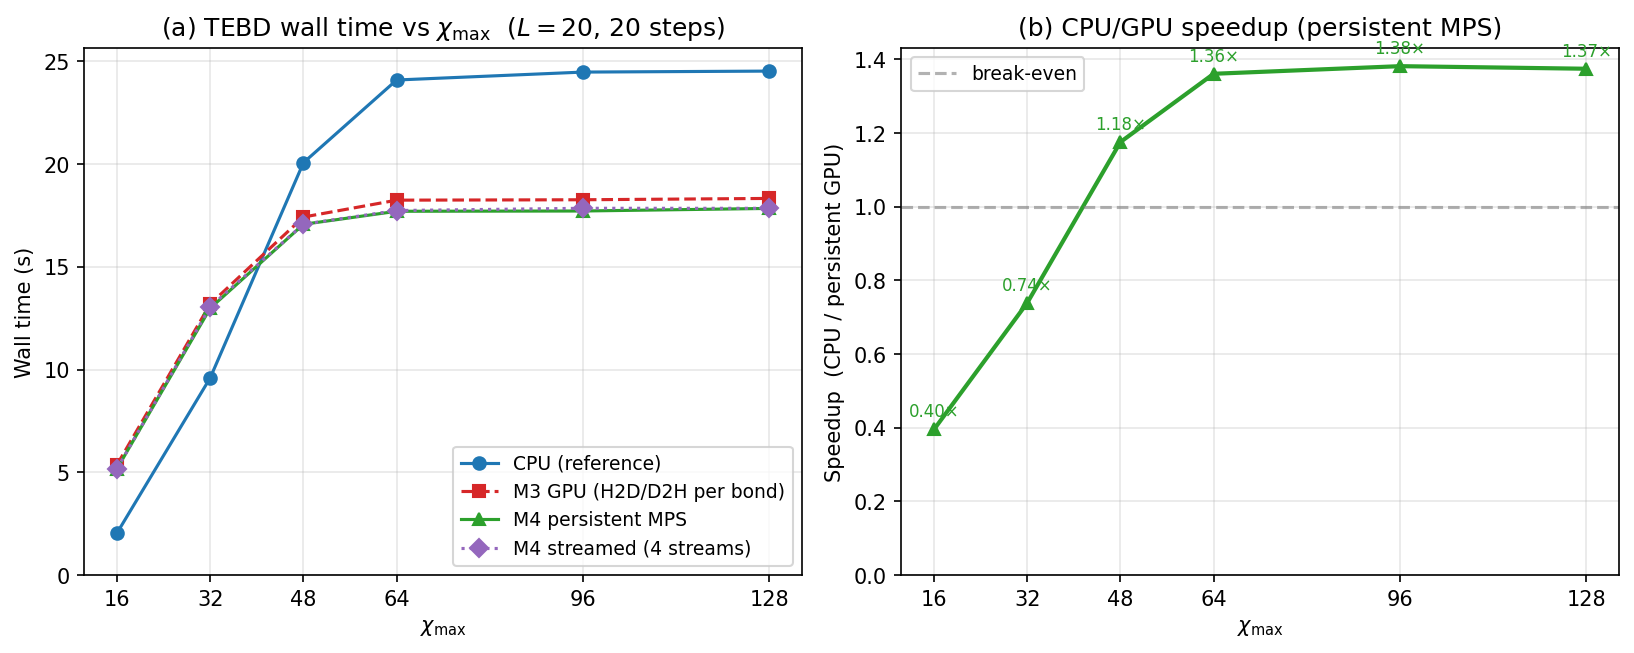
\includegraphics[width=0.92\textwidth]{m4_gpu_timing.png}
\caption{M4 single-GPU timing.  Persistent MPS consistently beats the M3
host-staging path; four streams yield negligible improvement.}
\label{fig:m4gpu}
\end{figure}

\textbf{Nsight Systems profiling.}
We ran two Nsight profiles.

\emph{Single-GPU} (\code{bench\_gpu}, $L{=}20$, $\chi_{\max}{=}64$, 3 steps),
profiled with \code{nsys profile --stats=true}.  Kernel-time shares below come
from \texttt{cuda\_gpu\_kern\_sum}.

\emph{Multi-GPU distributed} (\code{sweep\_mpi}, 4 ranks, $\chi_{\max}{=}64$,
3 steps/pair), launched under \code{mpirun -n 4 nsys profile --stats=true}
with a per-rank output name, giving one Nsight report per rank.

Distributed-profile findings:
\begin{itemize}
  \item \emph{Uniform compute.}  Every rank spends $96.2$--$96.5\%$ of GPU
    kernel time in the three main cuSOLVER Jacobi kernels, matching the
    single-GPU profile.
  \item \emph{No MPI in the timeline.}  No MPI calls appear in Nsight; the
    final \code{MPI\_Gatherv} ($\lesssim10$\,KB) is below profiler resolution.
  \item \emph{Memory traffic follows pair count.}  Per-rank H2D/D2H traffic
    ($\approx23$/$65$\,MB) comes from loading and finishing four independent
    pairs, not from distributed communication.
\end{itemize}

\begin{table}[h]
\centering\small
\begin{tabular}{lrl}
\toprule
\textbf{GPU kernel group} & \textbf{Share of kernel time} & \textbf{Note} \\
\midrule
cuSOLVER gesvdbj + svd\_col/row\_rotate & $96.4\%$ & top-3 Jacobi SVD kernels \\
All remaining cuSOLVER helpers & $3.2\%$ & sort, scale, QR, etc. \\
gate\_contract\_kernel (ours) & $0.09\%$ & \\
vidal\_restore left+right (ours) & $0.13\%$ & \\
theta2 + ss\_inv kernels (ours) & $0.11\%$ & persistent-path only \\
row\_to\_col\_kernel (ours) & $0.06\%$ & \\
\textbf{MPI communication} & $\mathbf{< 0.01\%}$ & \code{Gatherv} of $\sim$10\,KB at end \\
\bottomrule
\end{tabular}
\caption{Single-GPU per-stage GPU kernel-time breakdown.}
\label{tab:breakdown}
\end{table}

\textbf{Computation vs.\ communication.}
GPU kernels are $>99\%$ of wall time; cuSOLVER Jacobi alone is $>99.6\%$ of
GPU kernel time and our custom kernels together $<0.4\%$.  The final
\code{MPI\_Gatherv} ($\lesssim10$\,KB/rank) is negligible, and profiled PCIe
traffic ($\approx0.24$\,MB H2D, $0.18$\,MB D2H) confirms persistent MPS
removes M3's bulk tensor transfers.

\textbf{MPI scaling.}
Table~\ref{tab:mpi} and Figure~\ref{fig:mpi} use total rank wall time
$= \max_r \sum_{i\in{\rm rank}(r)} t_i$, the maximum sequential
pair-processing time over ranks; \code{sweep\_mpi} reports this directly as
\code{t\_rank\_max\_s}.

\begin{table}[h]
\centering
\setlength{\tabcolsep}{5pt}
\renewcommand{\arraystretch}{0.85}
\small
\begin{tabular}{rrrrrr}
\toprule
Mode & Ranks & Pairs/rank & Time (s) & Speedup & Eff. \\
\midrule
strong & 1 & 16 & 321.6 & 1.00 & 100\% \\
strong & 2 &  8 & 184.3 & 1.75 &  87\% \\
strong & 4 &  4 &  99.1 & 3.24 &  81\% \\
\midrule
weak   & 1 &  4 &  17.1 & --- & 100\% \\
weak   & 2 &  4 &  59.1 & --- &  29\% \\
weak   & 4 &  4 & 103.5 & --- &  17\% \\
\bottomrule
\end{tabular}
\caption{MPI scaling. Strong speedup relative to 1-rank total (321.6\,s).}
\label{tab:mpi}
\end{table}

\begin{figure}[!ht]
\centering
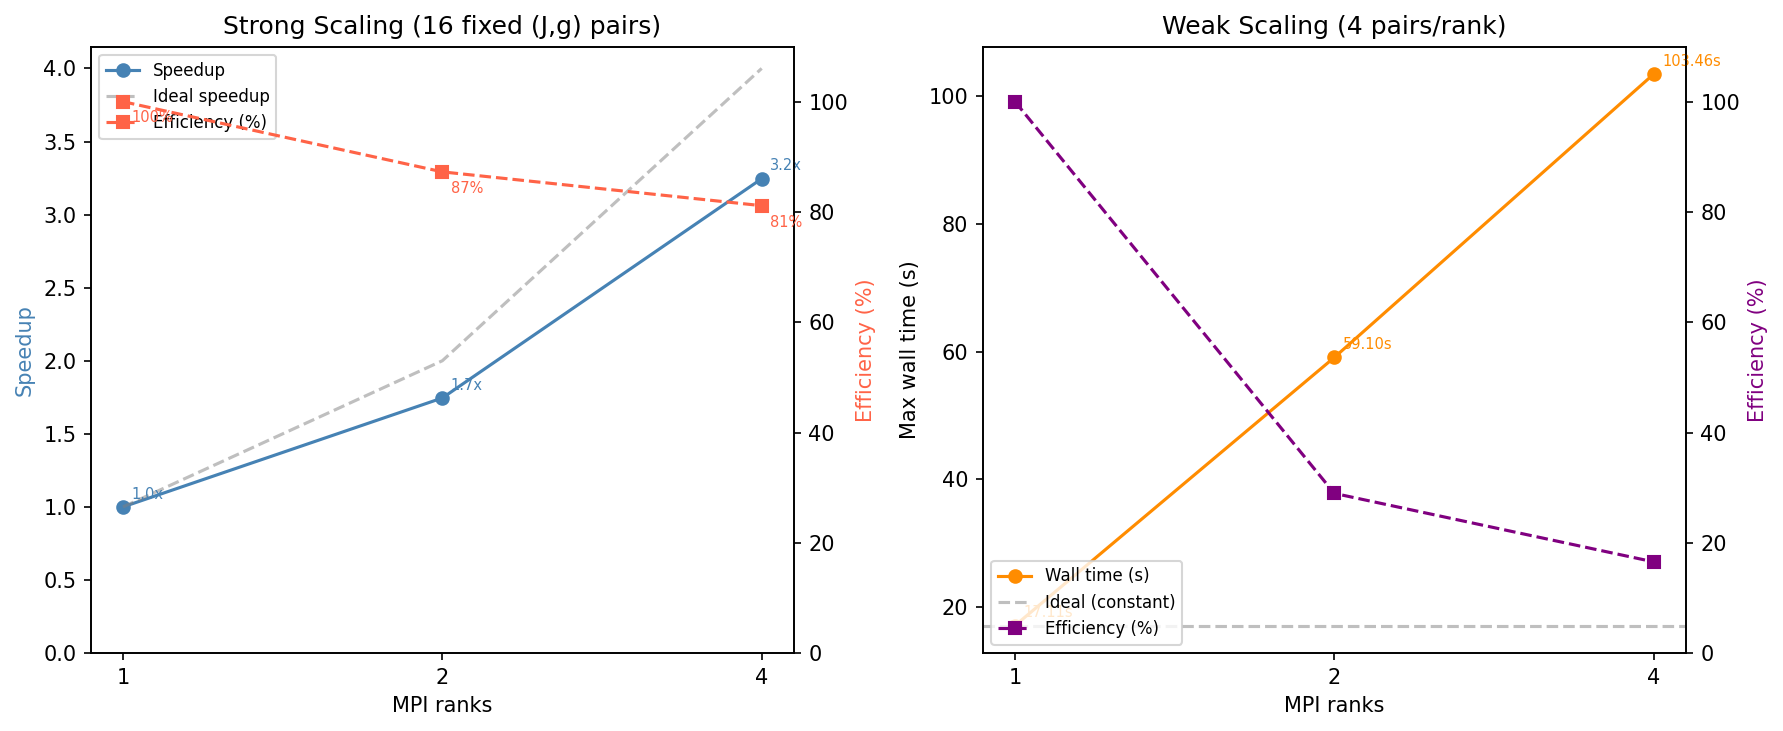
\includegraphics[width=0.7\textwidth]{scaling_m4.png}
\caption{Left: strong-scaling speedup (efficiency annotated).
Right: weak-scaling total rank wall time with efficiency.}
\label{fig:mpi}
\end{figure}

\textbf{cuSOLVER vs.\ custom Jacobi SVD.}
Table~\ref{tab:svd} and Figure~\ref{fig:svd} compare the two SVD paths.

\begin{table}[h]\centering\small
\begin{tabular}{rrrrr}
\toprule
$\chi_{\max}$ & cuSOLVER (s) & Jacobi (s) & Ratio & max $|\Delta\sigma|$ \\
\midrule
16  & 5.318 & 6.125  & 0.868 & $4.74\times10^{-14}$ \\
32  & 13.028 & 20.441 & 0.637 & $5.84\times10^{-13}$ \\
64  & 18.272 & 39.982 & 0.457 & $1.00\times10^{-12}$ \\
128 & 18.458 & 40.343 & 0.458 & $1.00\times10^{-12}$ \\
\bottomrule
\end{tabular}
\caption{\code{bench\_svd}: cuSOLVER vs.\ custom Jacobi, $L=20$, 20 steps.}
\label{tab:svd}
\end{table}

\begin{figure}[!ht]\centering
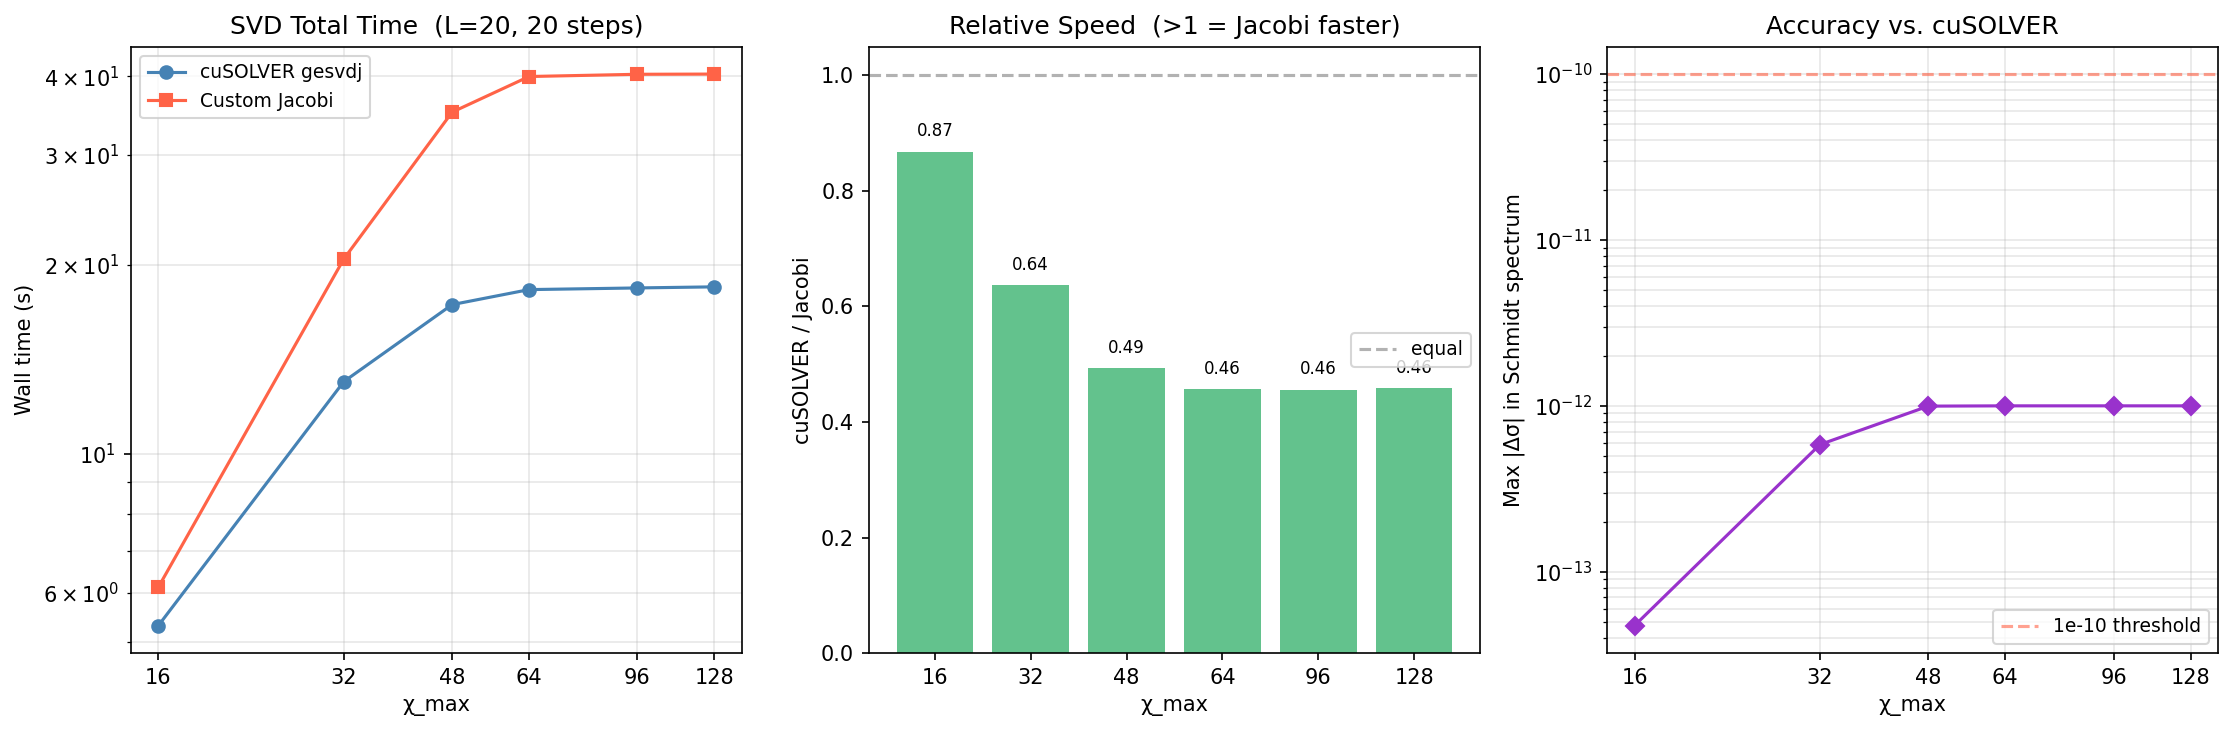
\includegraphics[width=0.92\textwidth]{svd_compare.png}
\caption{Custom Jacobi is 1.2--2.2$\times$ slower than cuSOLVER; accuracy
is $\lesssim10^{-12}$ after fixing the wide-matrix adjoint case.}
\label{fig:svd}
\end{figure}

\textbf{Scalability bottlenecks.}
\begin{itemize}
  \item \emph{Compute bottleneck (single GPU).}  cuSOLVER Jacobi SVD kernels
    account for $>99.6\%$ of GPU kernel time.  Persistent MPS and stream
    overlap cannot move the ceiling because SVD dominates.
  \item \emph{Load imbalance (strong scaling).}  Round-robin assignment gives
    rank 3 the four hardest pairs ($J{=}2.0$, all $g$), which run $2.2\times$
    longer than rank 0's cheapest pairs.  This explains the 19\% efficiency
    gap at $P{=}4$; communication is $<0.01\%$.
  \item \emph{Non-uniform work (weak scaling).}  Each added rank receives
    higher-$J$ pairs with more entanglement and higher cost, so efficiency
    falls despite zero in-loop communication.
\end{itemize}

\section{Discussion of approaches and bottlenecks}

\textbf{What worked well.}  Task-parallel MPI is the right design at this
scale: zero in-loop communication gives 81\% strong-scaling efficiency at
4 ranks, limited by load imbalance.  Persistent MPS also removes the M3 PCIe
bottleneck.

\textbf{What we would do differently.}
\begin{itemize}
  \item \emph{Load-balanced assignment.}  Round-robin ignores the large
    runtime spread ($5$\,s for $J{=}0.25$ vs.\ $32$\,s for $J{=}2.0$).
    Sorting by estimated $\chi_{\rm active}$ and bin-packing to ranks should
    raise strong-scaling efficiency to $\gtrsim95\%$.
  \item \emph{CUDA-aware MPI.}  Currently we \code{sync\_to\_host} before
    gather.  CUDA-aware MPI could gather device buffers directly, though the
    $<10$\,KB transfer makes this immaterial here.
  \item \emph{Spatial decomposition for large chains.}  For $L\gg100$ the
    task-parallel approach may run out of distinct pairs.  A bond-cut spatial
    decomposition would then require one \code{MPI\_Allgather} per Trotter
    sub-step for the boundary Schmidt spectrum ($\chi_{\max}$ doubles).
\end{itemize}

\textbf{Scalability limits.}  Strong mode exhausts the 16-pair grid at
16 ranks; beyond that, ranks idle.  Weak mode gives later ranks harder
pairs (larger $J$, higher entanglement), so constant-work weak scaling would
require balancing by estimated entanglement, not pair count.

\section{Challenges and next steps}

\textbf{Completed challenges.}
Adding the adjoint fallback for $m<n$ matrices fixed the wide-matrix Jacobi
bug and reduced trajectory-level error by nine orders of magnitude.  The
custom kernel remains 1.2--2.2$\times$ slower than cuSOLVER, so cuSOLVER
stays the production backend.

\textbf{Updated timeline (M4 $\to$ Final Report, Jun 8).}

\begin{table}[h]
\centering\small
\begin{tabular}{p{2.8cm}p{10.4cm}}
\toprule
\textbf{Dates} & \textbf{Tasks} \\
\midrule
May 27--Jun 1 &
  Run \code{ncu} roofline on \code{bench\_gpu}; extend weak scaling to
  $P{=}8$; extend \code{bench\_svd} to $\chi_{\max}{=}256$; generate the
  entanglement-entropy heatmap from existing $(J,g)$ CSV data.
  (\emph{Multi-GPU Nsight Systems profile: done, see \S6.}) \\
\addlinespace
Jun 2--5 &
  Draft 6-page final report: consolidate benchmark and physics results,
  write analysis sections, and incorporate figures. \\
\addlinespace
Jun 6--7 &
  Internal review; revise report; verify \code{submit\_all.sh}
  reproduces all figures from a clean build. \\
\addlinespace
\textbf{Jun 8} &
  \textbf{Final submission on Gradescope.} \\
\bottomrule
\end{tabular}
\end{table}

\textbf{Stretch goal.}
Add $\langle\sigma^z_i\rangle$, $\langle\sigma^x_i\rangle$, and two-point
correlations to \code{sweep\_mpi.cpp}; rerun the phase-diagram sweep; plot
observable heatmaps.  This was planned in M1/M2 but still needs GPU-side
measurement code.

\textbf{Build and run.}  Build with \code{make -f Makefile.local}; jobs are
submitted via \code{sbatch} on \code{gpu-turing}---1 GPU for \code{validate\_gpu},
\code{bench\_gpu}, and \code{bench\_svd}, and 4 GPUs for the
\code{mpirun -n 4 ./apps/sweep\_mpi} sweep.

\end{document}